\section{Python} \label{sec:python}

We will now discuss the technologies employed in the development the the project (section \ref{sec:python}) as well as presenting our implementation of the algorithm Raft (section \ref{sec:raft}).

Python is a high-level, dynamically typed and interpreted programming language that is often used for scripting, data analysis and developing small applications, making it a non-obvious choice for this project, which is nothing of the above. 

As a language, it has two main of advantages compared to others: first of all it is undoubtedly the most popular and widely used in the world (figure \ref{fig:tiobe}) \cite{tiobe,ieeeSpect} which translates to abundant documentation and resources, and secondly it has a huge ecosystem of libraries that implement all the functionalities we need for this project, namely: \textit{xmlrpc} for the remote procedure calls (RPCs), \textit{threading} to handle local concurrency and \textit{Pygame} to manage everything game-related.

\begin{figure}[h]
  \centering
  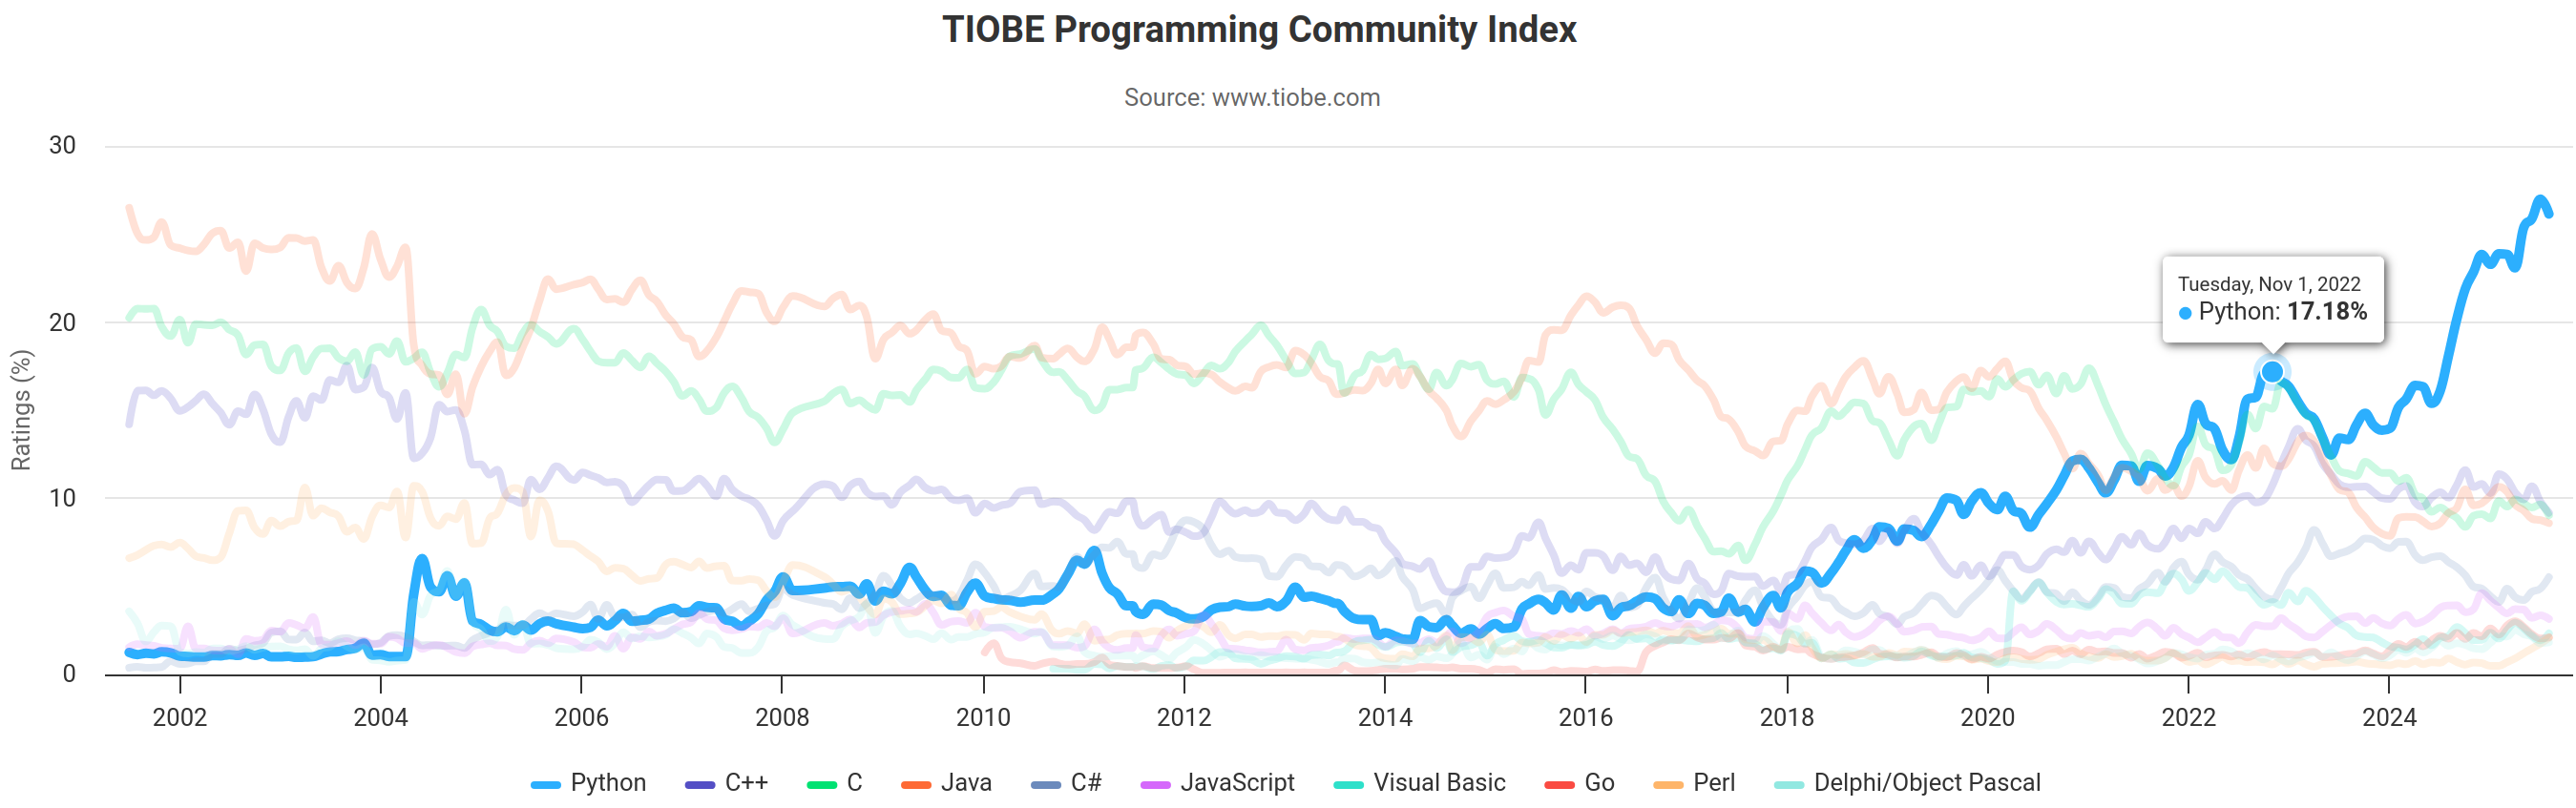
\includegraphics[width=\linewidth]{images/TIOBEindex.png}
  \caption{TIOBE Programming Community Index, focus on Python statistics, 2025. (\url{https://www.tiobe.com/tiobe-index/}).}
  \Description{Graph shows that Python gained populary since 2018 onwards becoming the most popular programming language.}
  \label{fig:tiobe}
\end{figure}


\subsection{Remote Procedure Calls} \label{sec:xmlrpc}

In Raft's specifications it is stated that nodes communicate with each other via remote procedure calls \cite{raft}, which in distributed computing is when a program causes a procedure (or subroutine) to execute in another address space (commonly on another computer on a shared network) calling it as if it were local (that is, the programmer writes the same code whether the subroutine is local or remote).

There are many libraries that implement this functionality, like gRPC (\url{https://grpc.io/}) which is a high performance open source RPC framework used by many big players, like Netflix \footnote{Netflix Ribbon is an Inter Process Communication library built in software load balancers: \url{https://github.com/Netflix/ribbon}} and Cockroach Labs \footnote{Cockroach Labs is the company behind CockroachDB, a highly resilient distributed database: \url{https://www.cockroachlabs.com/}}, available for many languages (Python included), but we opted for the standard library \textit{xmlrpc} \footnote{XML-RPC is a Remote Procedure Call method that uses XML passed via HTTP as a transport: \url{https://docs.python.org/3/library/xmlrpc.html}} thanks to its promised simplicity and ease of use. 

The library provides both server and client implementations, encapsulating the former in its own loop, while the latter can be fired as needed allowing a bit more flexibility in its usage.

In the following code \verb|client| encapsulates a server living in its own networked location and is used to call the remote procedure \verb|test_foo| like it was a local one.

\begin{python}
with xmlrpc.client.ServerProxy('http://localhost:8000', allow_none=True) as client:
    print(client.test_foo(42)) # print returned value
\end{python}

The server must be instantiated and left alive, and all remote procedure calls registered with \verb|register_function|.

\begin{python}
with SimpleXMLRPCServer (('localhost', 8000)) as server:
    def test_foo(number):
        return f'The number is {number}'

    server.register_function(test_foo)  
    server.serve_forever() # keep server alive
\end{python}

For this project we extend \textit{SimpleXMLRPCServer} to create a class that implements the Raft protocol (more details in section \ref{sec:implementation})

\subsection{Concurrency} \label{sec:threading}

In this project the need for concurrent programming arises from two challenges: every server have an internal timer that fires at certain intervals, and every node have to run a game engine and the server itself at the same time, both of which can be simplified as two \textit{"while true"} loops. 

Most Raft implementations achieve concurrency with asynchronous programming, using libraries such as \textit{asyncio} \footnote{asyncio is a library to write concurrent code using the async/await syntax: \url{https://docs.python.org/3/library/asyncio.html}}, which while powerful and efficient, makes writing code a bit awkward and cumbersome. We thus opted for a more traditional approach using multithreaded programming: in computer science, a thread of execution is the smallest sequence of programmed instruction that can be managed independently by the scheduler \cite{lamportMultiprocessor}, and multiple threads may be executed concurrently sharing resources such as memory, which is directly counterpointed to multiprocessing where each process has its own storage space (moreover, processes are typically made of threads). 

In Python there are modules in the standard library for both of them, respectively \textit{threading} \footnote{The threading module provides a way to run multiple threads (smaller units of a process) concurrently within a single process: \url{https://docs.python.org/3/library/threading.html}} and \textit{multiprocessing} \footnote{The multiprocessing module is a package that supports spawning processes using an API similar to the threading module: \url{https://docs.python.org/3/library/multiprocessing.html}}. It is fundamental to note that the former does not provide real multi-threading since, due to the Global Interpreter Lock of CPython (the, for want of a better word, "official" Python implementation), only one thread can execute bytecode at once. To cite directly from the documentation: \textit{"[GIL is] The mechanism used by the CPython interpreter to assure that only one thread executes Python bytecode at a time. This simplifies the CPython implementation by making the object model (including critical built-in types such as dict) implicitly safe against concurrent access. Locking the entire interpreter makes it easier for the interpreter to be multi-threaded, at the expense of much of the parallelism afforded by multi-processor machines."} \footnote{Global Interpreter Lock: \url{https://docs.python.org/3/glossary.html\#term-global-interpreter-lock}}.

Thankfully, this does not apply with the \textit{multiprocessing} module, which creates separate processes instead, offering both local and remote concurrency effectively side-stepping the Global Interpreter Lock, allowing programmers to fully leverage multi-processors machines. As previously stated, processes are much heavier than threads and thus more expensive to create, but do not incur the risks of shared memory. 

\subsubsection{Comparison}

To evaluate which of the two modules is more suited for our purposes, we devised a simple experiment: we created two game instances with one hundred and one thousands coloured dots respectively (figure \ref{fig:randomdots}), that move around the screen offsetting their position each frame by a random amount between minus five and plus five pixels (pseudocode \ref{code:randomdots}).

Then we ran both of them in various scenarios: with the game instance alone (baselines), with a server alive in a thread and with a server alive in a process, and we measured the \textit{frames per second} (FPS) \footnote{Frame rate, most commonly expressed in frames per second or FPS, is typically the frequency (rate) at which consecutive images (frames) are captured or displayed. This definition applies to film and video cameras, computer animation, and motion capture systems, while in the context of computer graphics is the rate at which a system, particularly the graphic card, si able to generate frames. Source: \url{https://en.wikipedia.org/wiki/Frame_rate}} in each case, since it is the most common metric to evaluate game performance. Higher FPS-count translates to a smoother and more responsive, i.e., better, gaming experience.

\label{code:randomdots}
\begin{python} 
# create random offsets for both x and y coordinates
xmov = random.randint(-5,5)
ymov = random.randint(-5,5)

# move the dot by a certain offset
dot.move_by(xmov, ymov)
\end{python}

\begin{figure}[h]
  \centering
  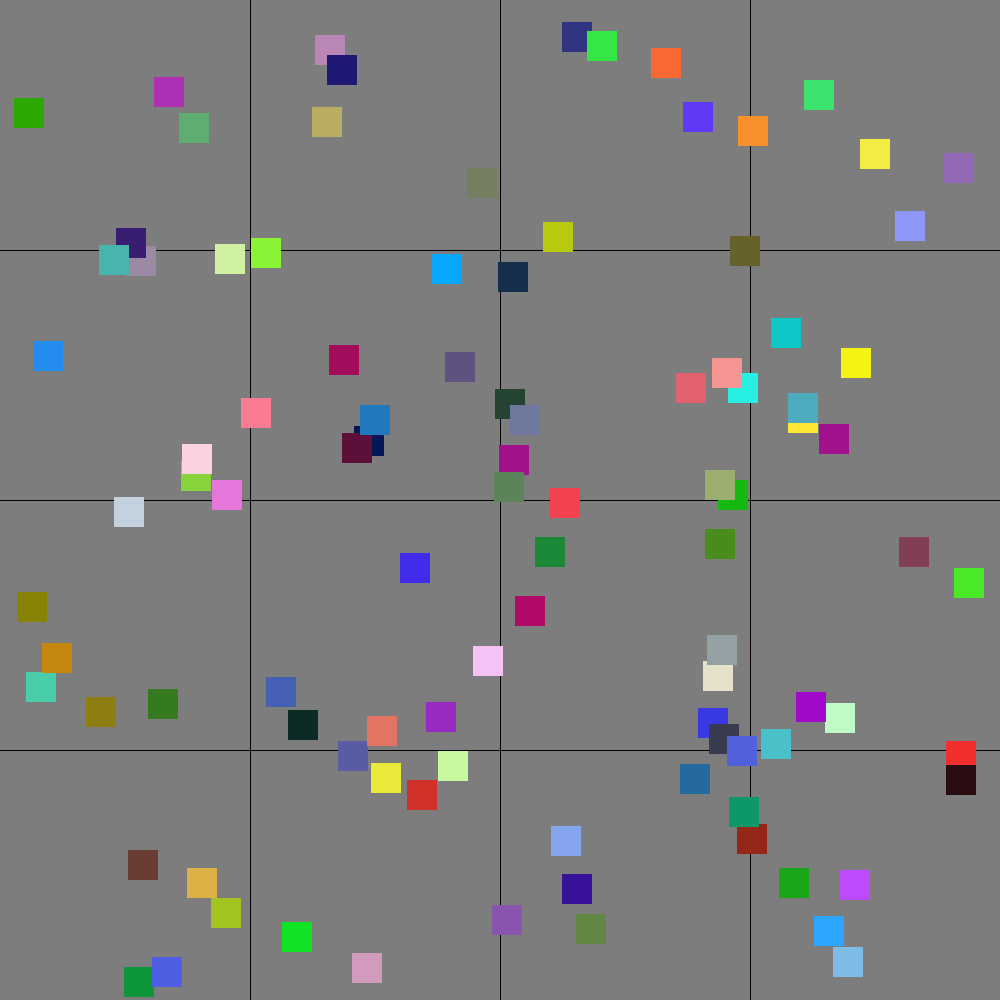
\includegraphics[width=.4\linewidth]{images/100dots.png}
  \hspace{.05\linewidth}
  
\includegraphics[width=.4\linewidth]{images/1000dots.png}
  
  \caption{Two game instances made with Pygame, with respectively 100 and 1000 dots that randomly move around.}
  \Description{Graph shows two game instances with respectively 100 and 1000 little colored squares that, once fired up, move around by a random offset.}
  \label{fig:randomdots}
\end{figure}

Results, shown in the graph at figure \ref{fig:peval} shows us that: 

\begin{itemize}
    \item Increasing the number of dots from 100 to 1000 halves the FPS count;
    \item Adding a server in a separate thread halves performances;
    \item Using \textit{multiprocessing} yields worse performances than \textit{threading} in the 100-dots scenario (about -30\%) while performs similarly in the 1000-dots one.
\end{itemize}

This leads us to conclude that, for our specific purposes, the \textit{threading} module is the best choice, especially since the final game will be way less computationally expensive from a graphical standpoint, hence using a lighter weight alternative should be even more beneficial than tested.

\begin{figure}[h]
  \centering
  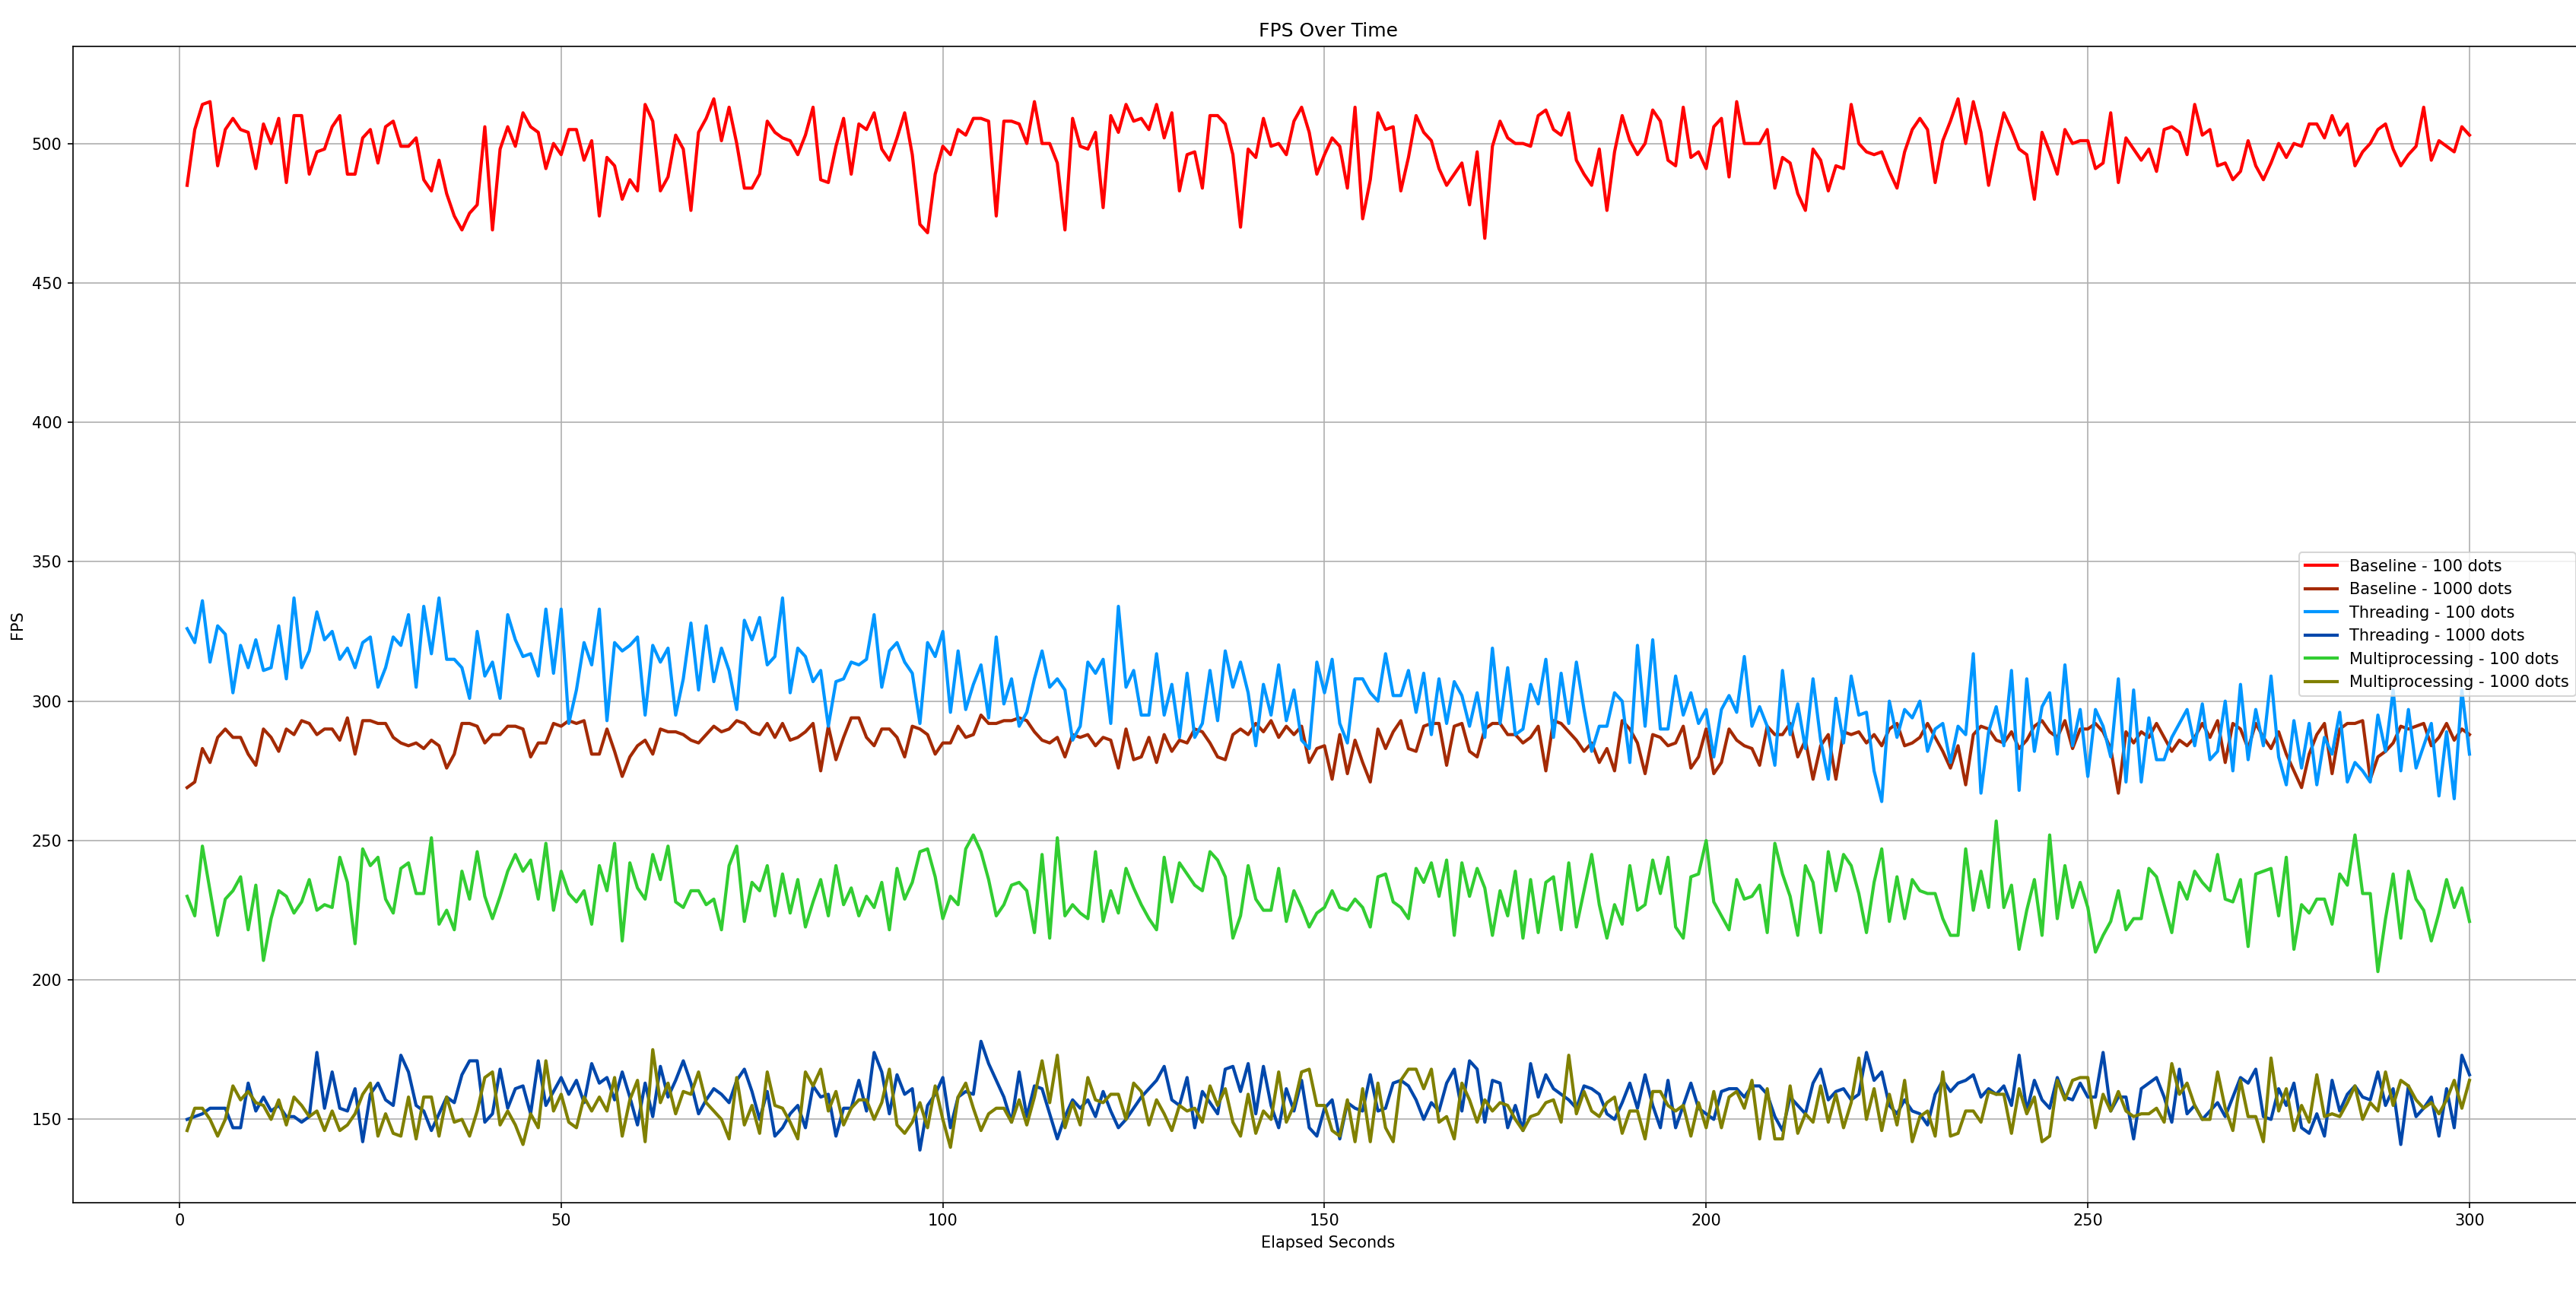
\includegraphics[width=\linewidth]{images/performance_eval_fps_graph.png}
  \caption{Performance evaluation graph: red hues for baselines, blue hues for threading and green hues for multiprocessing. Darker shades for 1000 dots and lighter shades for 100 dots game instances.}
  \Description{Line graph that shows that increasing the graphical load by 10x halves performances, and that module trheading performs 30\% better than multithreading in a low-demanding scenario.}
  \label{fig:peval}
\end{figure}

All tests have been performed with the following machine: 

\begin{itemize}
    \item OS: Ubuntu 24.04.1 LTS x86\_64;
    \item Kernel: 6.8.0-52-generic;
    \item Shell: bash 5.2.21;
    \item CPU: 13th Gen Intel i7-13620H;
    \item GPU: NVIDIA GeForce RTX 4050 Laptop GPU;
    \item Memory: 15610MiB;
    \item Python version: 3.12.3;
    \item Power Mode: Balanced;
    \item Alimentation: 100W via type C.
\end{itemize}

\subsection{Game Engine} \label{sec:pygame}

There are many ways to implement a graphical user interface: from clever shell tricks like htop \footnote{htop is a cross-platform text-mode interactive process viewer: \url{https://htop.dev/}}, to full fledged game engines like Unity \footnote{Unity is a cross-platform game engine developed by Unity Technologies: \url{https://unity.com/}}, we really had the luxury, and challenge, of choice.

More serious solutions like Godot (robust, open-source, based on C++, allows even 3D development) or Phaser (lightweight and easy to use, based on JavaScript), come with their own editor and have a \textit{top-down} approach, meaning the developer is supposed to build the graphical components first, and then go down to code as needed for scripting and refining. This is not optimal for our needs since it would make it more challenging to implement the Raft protocol.

What we wanted was a \textit{bottom-up} approach, where everything stems from the code itself to simplify merging all project's components, better yet if using the same programming language. Python offers exactly this since not only natively supports both RPCs and concurrency (as previously stated) but also has a module in the standard library that handles graphical user interfaces (UIs), namely tkinter, and the community-developed framework Pygame.

\subsubsection{Comparison}

Deciding between tkinter and Pygame ultimately came down to ease of development, power and flexibility. Let's briefly list the strengths and weaknesses of both: tkinter, being part of the standard library, is very well documented and supported, but since tis made to develop static UIs of simple applications it does not support advanced 

That being said we ultimately decided to opt for the framework Pygame since it offers way more flexibility, easier to handle   